\documentclass[1p]{elsarticle_modified}
%\bibliographystyle{elsarticle-num}

%\usepackage[colorlinks]{hyperref}
%\usepackage{abbrmath_seonhwa} %\Abb, \Ascr, \Acal ,\Abf, \Afrak
\usepackage{amsfonts}
\usepackage{amssymb}
\usepackage{amsmath}
\usepackage{amsthm}
\usepackage{scalefnt}
\usepackage{amsbsy}
\usepackage{kotex}
\usepackage{caption}
\usepackage{subfig}
\usepackage{color}
\usepackage{graphicx}
\usepackage{xcolor} %% white, black, red, green, blue, cyan, magenta, yellow
\usepackage{float}
\usepackage{setspace}
\usepackage{hyperref}

\usepackage{tikz}
\usetikzlibrary{arrows}

\usepackage{multirow}
\usepackage{array} % fixed length table
\usepackage{hhline}

%%%%%%%%%%%%%%%%%%%%%
\makeatletter
\renewcommand*\env@matrix[1][\arraystretch]{%
	\edef\arraystretch{#1}%
	\hskip -\arraycolsep
	\let\@ifnextchar\new@ifnextchar
	\array{*\c@MaxMatrixCols c}}
\makeatother %https://tex.stackexchange.com/questions/14071/how-can-i-increase-the-line-spacing-in-a-matrix
%%%%%%%%%%%%%%%

\usepackage[normalem]{ulem}

\newcommand{\msout}[1]{\ifmmode\text{\sout{\ensuremath{#1}}}\else\sout{#1}\fi}
%SOURCE: \msout is \stkout macro in https://tex.stackexchange.com/questions/20609/strikeout-in-math-mode

\newcommand{\cancel}[1]{
	\ifmmode
	{\color{red}\msout{#1}}
	\else
	{\color{red}\sout{#1}}
	\fi
}

\newcommand{\add}[1]{
	{\color{blue}\uwave{#1}}
}

\newcommand{\replace}[2]{
	\ifmmode
	{\color{red}\msout{#1}}{\color{blue}\uwave{#2}}
	\else
	{\color{red}\sout{#1}}{\color{blue}\uwave{#2}}
	\fi
}

\newcommand{\Sol}{\mathcal{S}} %segment
\newcommand{\D}{D} %diagram
\newcommand{\A}{\mathcal{A}} %arc


%%%%%%%%%%%%%%%%%%%%%%%%%%%%%5 test

\def\sl{\operatorname{\textup{SL}}(2,\Cbb)}
\def\psl{\operatorname{\textup{PSL}}(2,\Cbb)}
\def\quan{\mkern 1mu \triangleright \mkern 1mu}

\theoremstyle{definition}
\newtheorem{thm}{Theorem}[section]
\newtheorem{prop}[thm]{Proposition}
\newtheorem{lem}[thm]{Lemma}
\newtheorem{ques}[thm]{Question}
\newtheorem{cor}[thm]{Corollary}
\newtheorem{defn}[thm]{Definition}
\newtheorem{exam}[thm]{Example}
\newtheorem{rmk}[thm]{Remark}
\newtheorem{alg}[thm]{Algorithm}

\newcommand{\I}{\sqrt{-1}}
\begin{document}

%\begin{frontmatter}
%
%\title{Boundary parabolic representations of knots up to 8 crossings}
%
%%% Group authors per affiliation:
%\author{Yunhi Cho} 
%\address{Department of Mathematics, University of Seoul, Seoul, Korea}
%\ead{yhcho@uos.ac.kr}
%
%
%\author{Seonhwa Kim} %\fnref{s_kim}}
%\address{Center for Geometry and Physics, Institute for Basic Science, Pohang, 37673, Korea}
%\ead{ryeona17@ibs.re.kr}
%
%\author{Hyuk Kim}
%\address{Department of Mathematical Sciences, Seoul National University, Seoul 08826, Korea}
%\ead{hyukkim@snu.ac.kr}
%
%\author{Seokbeom Yoon}
%\address{Department of Mathematical Sciences, Seoul National University, Seoul, 08826,  Korea}
%\ead{sbyoon15@snu.ac.kr}
%
%\begin{abstract}
%We find all boundary parabolic representation of knots up to 8 crossings.
%
%\end{abstract}
%\begin{keyword}
%    \MSC[2010] 57M25 
%\end{keyword}
%
%\end{frontmatter}

%\linenumbers
%\tableofcontents
%
\newcommand\colored[1]{\textcolor{white}{\rule[-0.35ex]{0.8em}{1.4ex}}\kern-0.8em\color{red} #1}%
%\newcommand\colored[1]{\textcolor{white}{ #1}\kern-2.17ex	\textcolor{white}{ #1}\kern-1.81ex	\textcolor{white}{ #1}\kern-2.15ex\color{red}#1	}

{\Large $\underline{12n_{0420}~(K12n_{0420})}$}

\setlength{\tabcolsep}{10pt}
\renewcommand{\arraystretch}{1.6}
\vspace{1cm}\begin{tabular}{m{100pt}>{\centering\arraybackslash}m{274pt}}
\multirow{5}{120pt}{
	\centering
	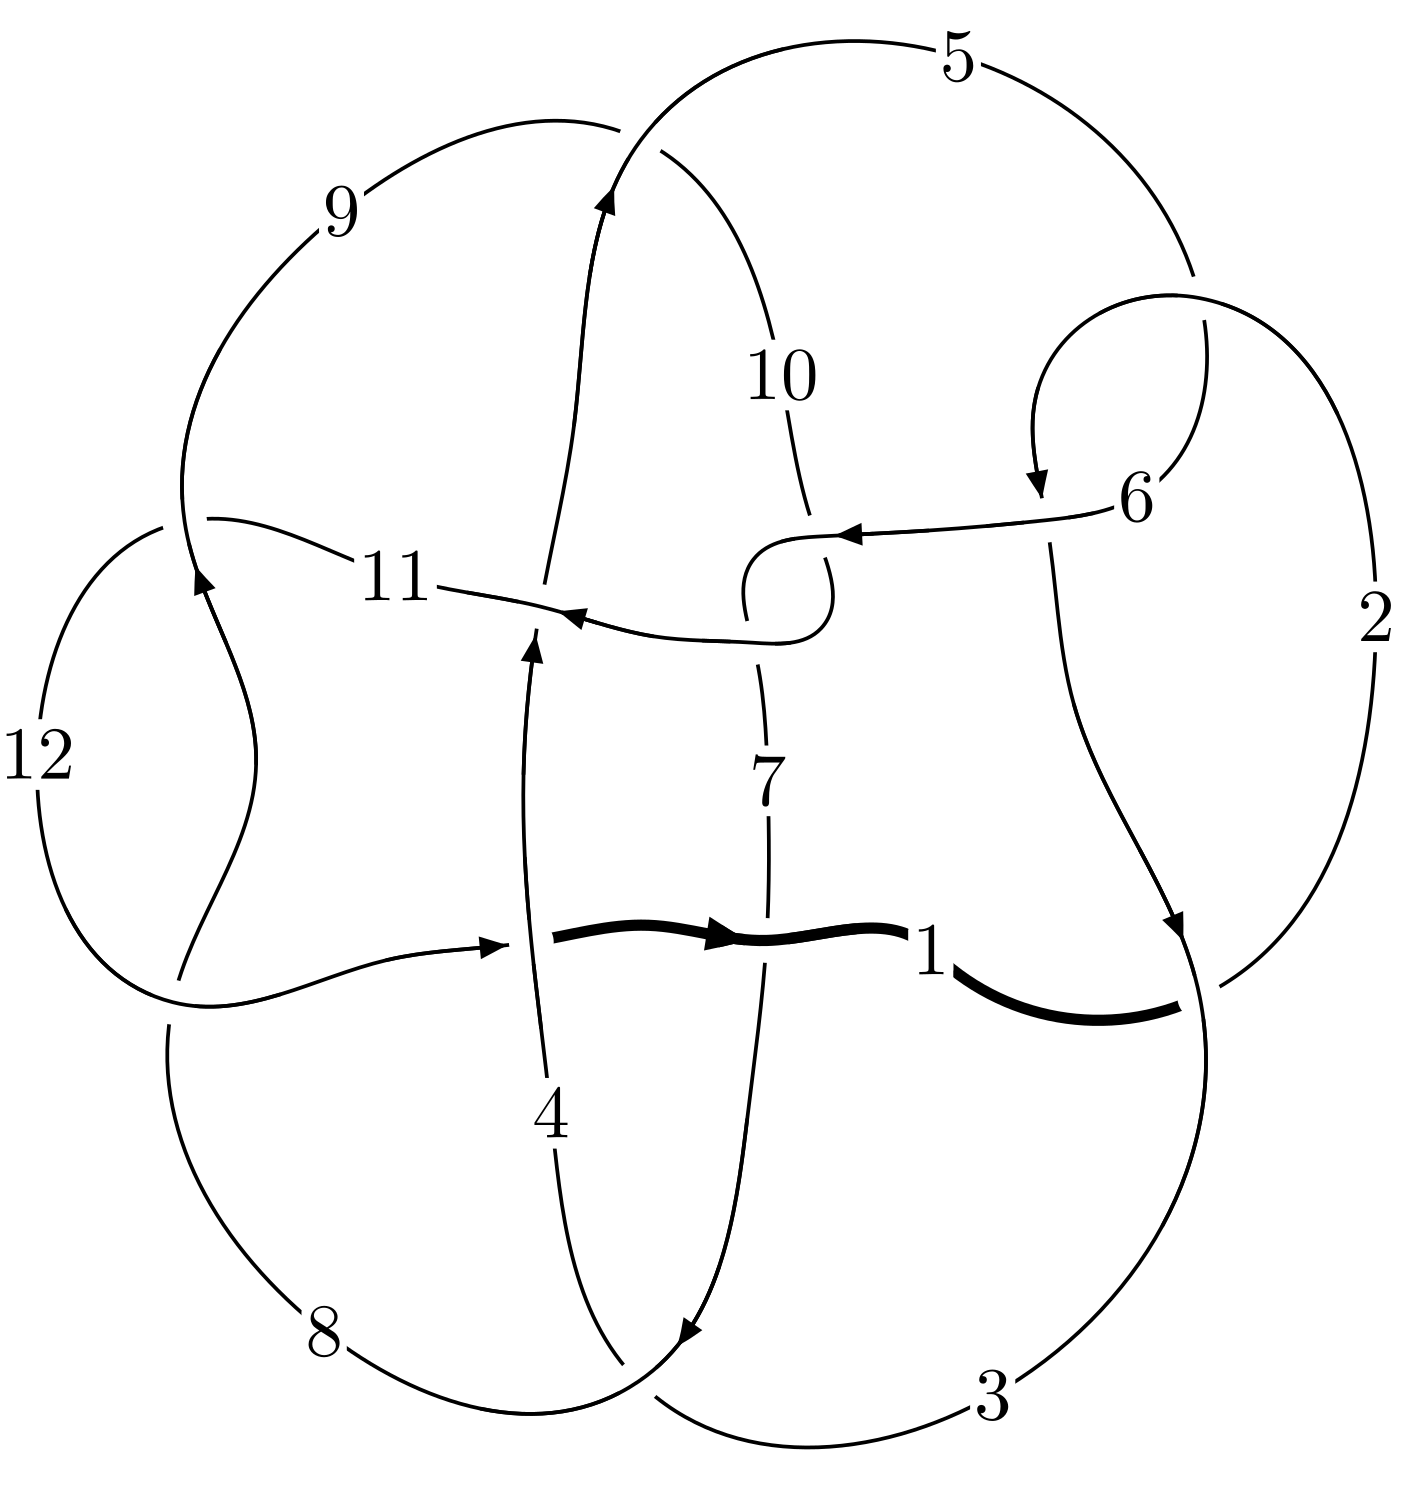
\includegraphics[width=112pt]{../../../GIT/diagram.site/Diagrams/png/2509_12n_0420.png}\\
\ \ \ A knot diagram\footnotemark}&
\allowdisplaybreaks
\textbf{Linearized knot diagam} \\
\cline{2-2}
 &
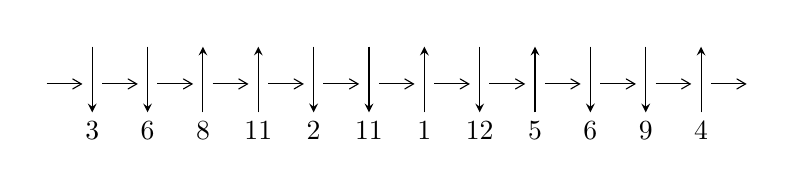
\begin{tikzpicture}[x=20pt, y=17pt]
	% nodes
	\node (C0) at (0, 0) {};
	\node (C1) at (1, 0) {};
	\node (C1U) at (1, +1) {};
	\node (C1D) at (1, -1) {3};

	\node (C2) at (2, 0) {};
	\node (C2U) at (2, +1) {};
	\node (C2D) at (2, -1) {6};

	\node (C3) at (3, 0) {};
	\node (C3U) at (3, +1) {};
	\node (C3D) at (3, -1) {8};

	\node (C4) at (4, 0) {};
	\node (C4U) at (4, +1) {};
	\node (C4D) at (4, -1) {11};

	\node (C5) at (5, 0) {};
	\node (C5U) at (5, +1) {};
	\node (C5D) at (5, -1) {2};

	\node (C6) at (6, 0) {};
	\node (C6U) at (6, +1) {};
	\node (C6D) at (6, -1) {11};

	\node (C7) at (7, 0) {};
	\node (C7U) at (7, +1) {};
	\node (C7D) at (7, -1) {1};

	\node (C8) at (8, 0) {};
	\node (C8U) at (8, +1) {};
	\node (C8D) at (8, -1) {12};

	\node (C9) at (9, 0) {};
	\node (C9U) at (9, +1) {};
	\node (C9D) at (9, -1) {5};

	\node (C10) at (10, 0) {};
	\node (C10U) at (10, +1) {};
	\node (C10D) at (10, -1) {6};

	\node (C11) at (11, 0) {};
	\node (C11U) at (11, +1) {};
	\node (C11D) at (11, -1) {9};

	\node (C12) at (12, 0) {};
	\node (C12U) at (12, +1) {};
	\node (C12D) at (12, -1) {4};
	\node (C13) at (13, 0) {};

	% arrows
	\draw[->,>={angle 60}]
	(C0) edge (C1) (C1) edge (C2) (C2) edge (C3) (C3) edge (C4) (C4) edge (C5) (C5) edge (C6) (C6) edge (C7) (C7) edge (C8) (C8) edge (C9) (C9) edge (C10) (C10) edge (C11) (C11) edge (C12) (C12) edge (C13) ;	\draw[->,>=stealth]
	(C1U) edge (C1D) (C2U) edge (C2D) (C3D) edge (C3U) (C4D) edge (C4U) (C5U) edge (C5D) (C6U) edge (C6D) (C7D) edge (C7U) (C8U) edge (C8D) (C9D) edge (C9U) (C10U) edge (C10D) (C11U) edge (C11D) (C12D) edge (C12U) ;
	\end{tikzpicture} \\
\hhline{~~} \\& 
\textbf{Solving Sequence} \\ \cline{2-2} 
 &
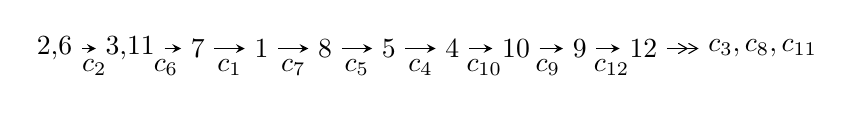
\begin{tikzpicture}[x=23pt, y=7pt]
	% node
	\node (A0) at (-1/8, 0) {2,6};
	\node (A1) at (17/16, 0) {3,11};
	\node (A2) at (17/8, 0) {7};
	\node (A3) at (25/8, 0) {1};
	\node (A4) at (33/8, 0) {8};
	\node (A5) at (41/8, 0) {5};
	\node (A6) at (49/8, 0) {4};
	\node (A7) at (57/8, 0) {10};
	\node (A8) at (65/8, 0) {9};
	\node (A9) at (73/8, 0) {12};
	\node (C1) at (1/2, -1) {$c_{2}$};
	\node (C2) at (13/8, -1) {$c_{6}$};
	\node (C3) at (21/8, -1) {$c_{1}$};
	\node (C4) at (29/8, -1) {$c_{7}$};
	\node (C5) at (37/8, -1) {$c_{5}$};
	\node (C6) at (45/8, -1) {$c_{4}$};
	\node (C7) at (53/8, -1) {$c_{10}$};
	\node (C8) at (61/8, -1) {$c_{9}$};
	\node (C9) at (69/8, -1) {$c_{12}$};
	\node (A10) at (11, 0) {$c_{3},c_{8},c_{11}$};

	% edge
	\draw[->,>=stealth]	
	(A0) edge (A1) (A1) edge (A2) (A2) edge (A3) (A3) edge (A4) (A4) edge (A5) (A5) edge (A6) (A6) edge (A7) (A7) edge (A8) (A8) edge (A9) ;
	\draw[->>,>={angle 60}]	
	(A9) edge (A10);
\end{tikzpicture} \\ 

\end{tabular} \\

\footnotetext{
The image of knot diagram is generated by the software ``\textbf{Draw programme}" developed by Andrew Bartholomew(\url{http://www.layer8.co.uk/maths/draw/index.htm\#Running-draw}), where we modified some parts for our purpose(\url{https://github.com/CATsTAILs/LinksPainter}).
}\phantom \\ \newline 
\centering \textbf{Ideals for irreducible components\footnotemark of $X_{\text{par}}$} 
 
\begin{align*}
I^u_{1}&=\langle 
364223527493 u^{32}-2361609064840 u^{31}+\cdots+171190334071 b+90526252853,\\
\phantom{I^u_{1}}&\phantom{= \langle  }671951659745 u^{32}-4453002864896 u^{31}+\cdots+342380668142 a-1160832184987,\\
\phantom{I^u_{1}}&\phantom{= \langle  }u^{33}-8 u^{32}+\cdots-11 u+2\rangle \\
I^u_{2}&=\langle 
- u^{18}-6 u^{17}+\cdots+b+3,\;2 u^{18}+7 u^{17}+\cdots+a+2,\;u^{19}+5 u^{18}+\cdots-2 u-1\rangle \\
I^u_{3}&=\langle 
u^{14} a+39 u^{14}+\cdots+a+69,\;12 u^{14} a+4 u^{14}+\cdots+19 a+12,\\
\phantom{I^u_{3}}&\phantom{= \langle  }u^{15}+3 u^{14}+3 u^{13}-4 u^{12}-9 u^{11}-2 u^{10}+11 u^9+5 u^8-6 u^7-2 u^6+10 u^5+3 u^4-5 u^3+3 u+1\rangle \\
I^u_{4}&=\langle 
b^2-3 b a+a-1,\;a^2+1,\;u-1\rangle \\
\\
\end{align*}
\raggedright * 4 irreducible components of $\dim_{\mathbb{C}}=0$, with total 86 representations.\\
\footnotetext{All coefficients of polynomials are rational numbers. But the coefficients are sometimes approximated in decimal forms when there is not enough margin.}
\newpage
\renewcommand{\arraystretch}{1}
\centering \section*{I. $I^u_{1}= \langle 3.64\times10^{11} u^{32}-2.36\times10^{12} u^{31}+\cdots+1.71\times10^{11} b+9.05\times10^{10},\;6.72\times10^{11} u^{32}-4.45\times10^{12} u^{31}+\cdots+3.42\times10^{11} a-1.16\times10^{12},\;u^{33}-8 u^{32}+\cdots-11 u+2 \rangle$}
\flushleft \textbf{(i) Arc colorings}\\
\begin{tabular}{m{7pt} m{180pt} m{7pt} m{180pt} }
\flushright $a_{2}=$&$\begin{pmatrix}1\\0\end{pmatrix}$ \\
\flushright $a_{6}=$&$\begin{pmatrix}0\\u\end{pmatrix}$ \\
\flushright $a_{3}=$&$\begin{pmatrix}1\\u^2\end{pmatrix}$ \\
\flushright $a_{11}=$&$\begin{pmatrix}-1.96259 u^{32}+13.0060 u^{31}+\cdots-22.5803 u+3.39047\\-2.12759 u^{32}+13.7952 u^{31}+\cdots-2.47506 u-0.528805\end{pmatrix}$ \\
\flushright $a_{7}=$&$\begin{pmatrix}1.18113 u^{32}-6.74280 u^{31}+\cdots-5.72215 u+4.99723\\2.30591 u^{32}-15.5550 u^{31}+\cdots+7.17397 u-1.80465\end{pmatrix}$ \\
\flushright $a_{1}=$&$\begin{pmatrix}- u^2+1\\- u^4\end{pmatrix}$ \\
\flushright $a_{8}=$&$\begin{pmatrix}-0.716291 u^{32}+1.55456 u^{31}+\cdots+4.09153 u+1.50206\\-7.10380 u^{32}+48.6587 u^{31}+\cdots-37.9303 u+6.10199\end{pmatrix}$ \\
\flushright $a_{5}=$&$\begin{pmatrix}u\\u\end{pmatrix}$ \\
\flushright $a_{4}=$&$\begin{pmatrix}-1.12478 u^{32}+8.81217 u^{31}+\cdots-10.8961 u+6.80188\\-1.14806 u^{32}+10.3781 u^{31}+\cdots-22.6370 u+4.15836\end{pmatrix}$ \\
\flushright $a_{10}=$&$\begin{pmatrix}-1.96259 u^{32}+13.0060 u^{31}+\cdots-22.5803 u+3.39047\\0.996508 u^{32}-9.67025 u^{31}+\cdots+23.2414 u-5.91819\end{pmatrix}$ \\
\flushright $a_{9}=$&$\begin{pmatrix}-0.264402 u^{32}+4.24281 u^{31}+\cdots-27.6237 u+5.38349\\2.69469 u^{32}-18.4334 u^{31}+\cdots+18.1980 u-3.92517\end{pmatrix}$ \\
\flushright $a_{12}=$&$\begin{pmatrix}-1.35910 u^{32}+12.0492 u^{31}+\cdots-33.5143 u+3.10913\\3.64636 u^{32}-25.3633 u^{31}+\cdots+26.2232 u-4.54568\end{pmatrix}$\\&\end{tabular}
\flushleft \textbf{(ii) Obstruction class $= -1$}\\~\\
\flushleft \textbf{(iii) Cusp Shapes $= -\frac{71232541821}{171190334071} u^{32}+\frac{136288968420}{171190334071} u^{31}+\cdots+\frac{5957445668473}{171190334071} u-\frac{448061765060}{171190334071}$}\\~\\
\newpage\renewcommand{\arraystretch}{1}
\flushleft \textbf{(iv) u-Polynomials at the component}\newline \\
\begin{tabular}{m{50pt}|m{274pt}}
Crossings & \hspace{64pt}u-Polynomials at each crossing \\
\hline $$\begin{aligned}c_{1}\end{aligned}$$&$\begin{aligned}
&u^{33}+8 u^{32}+\cdots+13 u+4
\end{aligned}$\\
\hline $$\begin{aligned}c_{2},c_{5}\end{aligned}$$&$\begin{aligned}
&u^{33}+8 u^{32}+\cdots-11 u-2
\end{aligned}$\\
\hline $$\begin{aligned}c_{3},c_{12}\end{aligned}$$&$\begin{aligned}
&u^{33}-9 u^{31}+\cdots+11 u+1
\end{aligned}$\\
\hline $$\begin{aligned}c_{4}\end{aligned}$$&$\begin{aligned}
&u^{33}-16 u^{31}+\cdots+868 u+259
\end{aligned}$\\
\hline $$\begin{aligned}c_{6},c_{10}\end{aligned}$$&$\begin{aligned}
&u^{33}+u^{32}+\cdots+29 u+2
\end{aligned}$\\
\hline $$\begin{aligned}c_{7}\end{aligned}$$&$\begin{aligned}
&u^{33}-29 u^{32}+\cdots-159744 u+16384
\end{aligned}$\\
\hline $$\begin{aligned}c_{8},c_{11}\end{aligned}$$&$\begin{aligned}
&u^{33}-11 u^{32}+\cdots-57 u+4
\end{aligned}$\\
\hline $$\begin{aligned}c_{9}\end{aligned}$$&$\begin{aligned}
&u^{33}+u^{32}+\cdots+2 u+1
\end{aligned}$\\
\hline
\end{tabular}\\~\\
\newpage\renewcommand{\arraystretch}{1}
\flushleft \textbf{(v) Riley Polynomials at the component}\newline \\
\begin{tabular}{m{50pt}|m{274pt}}
Crossings & \hspace{64pt}Riley Polynomials at each crossing \\
\hline $$\begin{aligned}c_{1}\end{aligned}$$&$\begin{aligned}
&y^{33}+40 y^{32}+\cdots-2383 y-16
\end{aligned}$\\
\hline $$\begin{aligned}c_{2},c_{5}\end{aligned}$$&$\begin{aligned}
&y^{33}-8 y^{32}+\cdots+13 y-4
\end{aligned}$\\
\hline $$\begin{aligned}c_{3},c_{12}\end{aligned}$$&$\begin{aligned}
&y^{33}-18 y^{32}+\cdots+59 y-1
\end{aligned}$\\
\hline $$\begin{aligned}c_{4}\end{aligned}$$&$\begin{aligned}
&y^{33}-32 y^{32}+\cdots+556584 y-67081
\end{aligned}$\\
\hline $$\begin{aligned}c_{6},c_{10}\end{aligned}$$&$\begin{aligned}
&y^{33}+53 y^{32}+\cdots+33 y-4
\end{aligned}$\\
\hline $$\begin{aligned}c_{7}\end{aligned}$$&$\begin{aligned}
&y^{33}-9 y^{32}+\cdots-1459617792 y-268435456
\end{aligned}$\\
\hline $$\begin{aligned}c_{8},c_{11}\end{aligned}$$&$\begin{aligned}
&y^{33}+23 y^{32}+\cdots+177 y-16
\end{aligned}$\\
\hline $$\begin{aligned}c_{9}\end{aligned}$$&$\begin{aligned}
&y^{33}-53 y^{32}+\cdots-8 y-1
\end{aligned}$\\
\hline
\end{tabular}\\~\\
\newpage\flushleft \textbf{(vi) Complex Volumes and Cusp Shapes}
$$\begin{array}{c|c|c}  
\text{Solutions to }I^u_{1}& \I (\text{vol} + \sqrt{-1}CS) & \text{Cusp shape}\\
 \hline 
\begin{aligned}
u &= -0.703285 + 0.636850 I \\
a &= \phantom{-}1.106170 + 0.251999 I \\
b &= \phantom{-}0.909144 - 1.059290 I\end{aligned}
 & \phantom{-}4.30952 + 3.14688 I & \phantom{-}2.88697 - 4.88211 I \\ \hline\begin{aligned}
u &= -0.703285 - 0.636850 I \\
a &= \phantom{-}1.106170 - 0.251999 I \\
b &= \phantom{-}0.909144 + 1.059290 I\end{aligned}
 & \phantom{-}4.30952 - 3.14688 I & \phantom{-}2.88697 + 4.88211 I \\ \hline\begin{aligned}
u &= -0.417059 + 1.000070 I \\
a &= -0.648249 - 0.662444 I \\
b &= -0.580122 + 0.953178 I\end{aligned}
 & \phantom{-}5.17920 - 2.64024 I & \phantom{-}3.71273 + 1.48167 I \\ \hline\begin{aligned}
u &= -0.417059 - 1.000070 I \\
a &= -0.648249 + 0.662444 I \\
b &= -0.580122 - 0.953178 I\end{aligned}
 & \phantom{-}5.17920 + 2.64024 I & \phantom{-}3.71273 - 1.48167 I \\ \hline\begin{aligned}
u &= \phantom{-}1.030280 + 0.369979 I \\
a &= -0.005672 - 0.234478 I \\
b &= -0.462951 - 0.491884 I\end{aligned}
 & -1.92686 - 1.50296 I & -0.206389 + 1.352839 I \\ \hline\begin{aligned}
u &= \phantom{-}1.030280 - 0.369979 I \\
a &= -0.005672 + 0.234478 I \\
b &= -0.462951 + 0.491884 I\end{aligned}
 & -1.92686 + 1.50296 I & -0.206389 - 1.352839 I \\ \hline\begin{aligned}
u &= \phantom{-}1.100340 + 0.181053 I \\
a &= \phantom{-}0.180870 + 0.010838 I \\
b &= \phantom{-}0.858956 - 0.643211 I\end{aligned}
 & -0.342656 + 0.092474 I & -4.88343 + 1.19512 I \\ \hline\begin{aligned}
u &= \phantom{-}1.100340 - 0.181053 I \\
a &= \phantom{-}0.180870 - 0.010838 I \\
b &= \phantom{-}0.858956 + 0.643211 I\end{aligned}
 & -0.342656 - 0.092474 I & -4.88343 - 1.19512 I \\ \hline\begin{aligned}
u &= -0.759456 + 0.391806 I \\
a &= \phantom{-}0.009616 + 1.198430 I \\
b &= \phantom{-}0.866202 + 1.049840 I\end{aligned}
 & \phantom{-}3.92702 + 0.90107 I & \phantom{-}3.65109 - 2.09842 I \\ \hline\begin{aligned}
u &= -0.759456 - 0.391806 I \\
a &= \phantom{-}0.009616 - 1.198430 I \\
b &= \phantom{-}0.866202 - 1.049840 I\end{aligned}
 & \phantom{-}3.92702 - 0.90107 I & \phantom{-}3.65109 + 2.09842 I\\
 \hline 
 \end{array}$$\newpage$$\begin{array}{c|c|c}  
\text{Solutions to }I^u_{1}& \I (\text{vol} + \sqrt{-1}CS) & \text{Cusp shape}\\
 \hline 
\begin{aligned}
u &= -1.075450 + 0.453106 I \\
a &= -0.361831 + 0.442964 I \\
b &= -0.063445 + 1.049590 I\end{aligned}
 & -1.12678 + 5.28243 I & -1.72426 - 8.87772 I \\ \hline\begin{aligned}
u &= -1.075450 - 0.453106 I \\
a &= -0.361831 - 0.442964 I \\
b &= -0.063445 - 1.049590 I\end{aligned}
 & -1.12678 - 5.28243 I & -1.72426 + 8.87772 I \\ \hline\begin{aligned}
u &= \phantom{-}0.617486 + 0.446217 I \\
a &= \phantom{-}0.750133 + 0.203711 I \\
b &= \phantom{-}0.207012 - 0.540399 I\end{aligned}
 & -0.66765 - 1.55785 I & -3.86335 + 5.45533 I \\ \hline\begin{aligned}
u &= \phantom{-}0.617486 - 0.446217 I \\
a &= \phantom{-}0.750133 - 0.203711 I \\
b &= \phantom{-}0.207012 + 0.540399 I\end{aligned}
 & -0.66765 + 1.55785 I & -3.86335 - 5.45533 I \\ \hline\begin{aligned}
u &= -0.268250 + 0.672707 I \\
a &= \phantom{-}0.777671 + 0.095093 I \\
b &= \phantom{-}0.068519 - 0.534112 I\end{aligned}
 & \phantom{-}1.35635 - 1.05663 I & \phantom{-}4.19428 + 2.46182 I \\ \hline\begin{aligned}
u &= -0.268250 - 0.672707 I \\
a &= \phantom{-}0.777671 - 0.095093 I \\
b &= \phantom{-}0.068519 + 0.534112 I\end{aligned}
 & \phantom{-}1.35635 + 1.05663 I & \phantom{-}4.19428 - 2.46182 I \\ \hline\begin{aligned}
u &= \phantom{-}0.868458 + 0.964205 I \\
a &= -1.45868 - 0.78756 I \\
b &= -0.48302 - 1.49770 I\end{aligned}
 & \phantom{-}12.95180 - 2.19664 I & \phantom{-}5.82474 + 2.27919 I \\ \hline\begin{aligned}
u &= \phantom{-}0.868458 - 0.964205 I \\
a &= -1.45868 + 0.78756 I \\
b &= -0.48302 + 1.49770 I\end{aligned}
 & \phantom{-}12.95180 + 2.19664 I & \phantom{-}5.82474 - 2.27919 I \\ \hline\begin{aligned}
u &= \phantom{-}0.916626 + 0.950177 I \\
a &= -1.06864 - 1.17969 I \\
b &= -0.08093 - 1.74309 I\end{aligned}
 & \phantom{-}9.06275 + 2.60903 I & \phantom{-}0.48775 - 2.35974 I \\ \hline\begin{aligned}
u &= \phantom{-}0.916626 - 0.950177 I \\
a &= -1.06864 + 1.17969 I \\
b &= -0.08093 + 1.74309 I\end{aligned}
 & \phantom{-}9.06275 - 2.60903 I & \phantom{-}0.48775 + 2.35974 I\\
 \hline 
 \end{array}$$\newpage$$\begin{array}{c|c|c}  
\text{Solutions to }I^u_{1}& \I (\text{vol} + \sqrt{-1}CS) & \text{Cusp shape}\\
 \hline 
\begin{aligned}
u &= \phantom{-}1.023220 + 0.876693 I \\
a &= \phantom{-}0.87894 + 1.19241 I \\
b &= \phantom{-}0.37002 + 2.13539 I\end{aligned}
 & \phantom{-}12.43740 - 4.58287 I & \phantom{-}4.99508 + 2.38247 I \\ \hline\begin{aligned}
u &= \phantom{-}1.023220 - 0.876693 I \\
a &= \phantom{-}0.87894 - 1.19241 I \\
b &= \phantom{-}0.37002 - 2.13539 I\end{aligned}
 & \phantom{-}12.43740 + 4.58287 I & \phantom{-}4.99508 - 2.38247 I \\ \hline\begin{aligned}
u &= \phantom{-}0.990802 + 0.915834 I \\
a &= \phantom{-}1.36449 + 0.89241 I \\
b &= \phantom{-}0.89932 + 1.99675 I\end{aligned}
 & \phantom{-}8.82668 - 9.47341 I & \phantom{-0.000000 -}0. + 6.83895 I \\ \hline\begin{aligned}
u &= \phantom{-}0.990802 - 0.915834 I \\
a &= \phantom{-}1.36449 - 0.89241 I \\
b &= \phantom{-}0.89932 - 1.99675 I\end{aligned}
 & \phantom{-}8.82668 + 9.47341 I & \phantom{-0.000000 } 0. - 6.83895 I \\ \hline\begin{aligned}
u &= -1.241080 + 0.559280 I \\
a &= -0.055515 - 0.655838 I \\
b &= -1.07954 - 1.10250 I\end{aligned}
 & \phantom{-}2.34090 + 8.49049 I & \phantom{-}2.07804 - 5.32543 I \\ \hline\begin{aligned}
u &= -1.241080 - 0.559280 I \\
a &= -0.055515 + 0.655838 I \\
b &= -1.07954 + 1.10250 I\end{aligned}
 & \phantom{-}2.34090 - 8.49049 I & \phantom{-}2.07804 + 5.32543 I \\ \hline\begin{aligned}
u &= \phantom{-}0.893546 + 1.073000 I \\
a &= \phantom{-}1.11701 + 1.10394 I \\
b &= -0.47751 + 1.72433 I\end{aligned}
 & \phantom{-}14.6502 + 8.3217 I & \phantom{-}2.61160 - 3.46041 I \\ \hline\begin{aligned}
u &= \phantom{-}0.893546 - 1.073000 I \\
a &= \phantom{-}1.11701 - 1.10394 I \\
b &= -0.47751 - 1.72433 I\end{aligned}
 & \phantom{-}14.6502 - 8.3217 I & \phantom{-}2.61160 + 3.46041 I \\ \hline\begin{aligned}
u &= \phantom{-}1.08079 + 0.94085 I \\
a &= -1.30612 - 0.84939 I \\
b &= -0.96271 - 2.44484 I\end{aligned}
 & \phantom{-}14.0051 - 15.6492 I & \phantom{-}1.72340 + 7.56042 I \\ \hline\begin{aligned}
u &= \phantom{-}1.08079 - 0.94085 I \\
a &= -1.30612 + 0.84939 I \\
b &= -0.96271 + 2.44484 I\end{aligned}
 & \phantom{-}14.0051 + 15.6492 I & \phantom{-}1.72340 - 7.56042 I\\
 \hline 
 \end{array}$$\newpage$$\begin{array}{c|c|c}  
\text{Solutions to }I^u_{1}& \I (\text{vol} + \sqrt{-1}CS) & \text{Cusp shape}\\
 \hline 
\begin{aligned}
u &= -0.530622\phantom{ +0.000000I} \\
a &= -2.30551\phantom{ +0.000000I} \\
b &= -1.44839\phantom{ +0.000000I}\end{aligned}
 & -2.29787\phantom{ +0.000000I} & -17.6560\phantom{ +0.000000I} \\ \hline\begin{aligned}
u &= \phantom{-}0.208352 + 0.257728 I \\
a &= -2.37744 - 2.48596 I \\
b &= -0.264747 + 1.039230 I\end{aligned}
 & \phantom{-}3.34739 - 0.13046 I & \phantom{-}5.79773 + 0.03563 I \\ \hline\begin{aligned}
u &= \phantom{-}0.208352 - 0.257728 I \\
a &= -2.37744 + 2.48596 I \\
b &= -0.264747 - 1.039230 I\end{aligned}
 & \phantom{-}3.34739 + 0.13046 I & \phantom{-}5.79773 - 0.03563 I\\
 \hline 
 \end{array}$$\newpage\newpage\renewcommand{\arraystretch}{1}
\centering \section*{II. $I^u_{2}= \langle - u^{18}-6 u^{17}+\cdots+b+3,\;2 u^{18}+7 u^{17}+\cdots+a+2,\;u^{19}+5 u^{18}+\cdots-2 u-1 \rangle$}
\flushleft \textbf{(i) Arc colorings}\\
\begin{tabular}{m{7pt} m{180pt} m{7pt} m{180pt} }
\flushright $a_{2}=$&$\begin{pmatrix}1\\0\end{pmatrix}$ \\
\flushright $a_{6}=$&$\begin{pmatrix}0\\u\end{pmatrix}$ \\
\flushright $a_{3}=$&$\begin{pmatrix}1\\u^2\end{pmatrix}$ \\
\flushright $a_{11}=$&$\begin{pmatrix}-2 u^{18}-7 u^{17}+\cdots+u-2\\u^{18}+6 u^{17}+\cdots-4 u-3\end{pmatrix}$ \\
\flushright $a_{7}=$&$\begin{pmatrix}-2 u^{17}-8 u^{16}+\cdots-4 u+1\\- u^{17}-4 u^{16}+\cdots-4 u^3-6 u^2\end{pmatrix}$ \\
\flushright $a_{1}=$&$\begin{pmatrix}- u^2+1\\- u^4\end{pmatrix}$ \\
\flushright $a_{8}=$&$\begin{pmatrix}- u^{18}-4 u^{17}+\cdots-4 u-1\\-3 u^{18}-12 u^{17}+\cdots+3 u+1\end{pmatrix}$ \\
\flushright $a_{5}=$&$\begin{pmatrix}u\\u\end{pmatrix}$ \\
\flushright $a_{4}=$&$\begin{pmatrix}- u^{17}-4 u^{16}+\cdots-2 u+1\\-4 u^{18}-17 u^{17}+\cdots+5 u+4\end{pmatrix}$ \\
\flushright $a_{10}=$&$\begin{pmatrix}-2 u^{18}-7 u^{17}+\cdots+u-2\\4 u^{18}+19 u^{17}+\cdots-8 u-6\end{pmatrix}$ \\
\flushright $a_{9}=$&$\begin{pmatrix}-3 u^{18}-14 u^{17}+\cdots+3 u+2\\3 u^{18}+12 u^{17}+\cdots-6 u-2\end{pmatrix}$ \\
\flushright $a_{12}=$&$\begin{pmatrix}-3 u^{18}-12 u^{17}+\cdots+5 u+3\\2 u^{18}+11 u^{17}+\cdots-3 u-5\end{pmatrix}$\\&\end{tabular}
\flushleft \textbf{(ii) Obstruction class $= 1$}\\~\\
\flushleft \textbf{(iii) Cusp Shapes $= -14 u^{18}-57 u^{17}-68 u^{16}+85 u^{15}+290 u^{14}+126 u^{13}-418 u^{12}-544 u^{11}+95 u^{10}+567 u^9+182 u^8-289 u^7-164 u^6+78 u^5+u^4-101 u^3-31 u^2+35 u+22$}\\~\\
\newpage\renewcommand{\arraystretch}{1}
\flushleft \textbf{(iv) u-Polynomials at the component}\newline \\
\begin{tabular}{m{50pt}|m{274pt}}
Crossings & \hspace{64pt}u-Polynomials at each crossing \\
\hline $$\begin{aligned}c_{1}\end{aligned}$$&$\begin{aligned}
&u^{19}-7 u^{18}+\cdots+8 u-1
\end{aligned}$\\
\hline $$\begin{aligned}c_{2}\end{aligned}$$&$\begin{aligned}
&u^{19}+5 u^{18}+\cdots-2 u-1
\end{aligned}$\\
\hline $$\begin{aligned}c_{3},c_{12}\end{aligned}$$&$\begin{aligned}
&u^{19}+2 u^{16}+\cdots+3 u+1
\end{aligned}$\\
\hline $$\begin{aligned}c_{4}\end{aligned}$$&$\begin{aligned}
&u^{19}-7 u^{17}+\cdots+2 u-1
\end{aligned}$\\
\hline $$\begin{aligned}c_{5}\end{aligned}$$&$\begin{aligned}
&u^{19}-5 u^{18}+\cdots-2 u+1
\end{aligned}$\\
\hline $$\begin{aligned}c_{6}\end{aligned}$$&$\begin{aligned}
&u^{19}+u^{18}+\cdots- u-1
\end{aligned}$\\
\hline $$\begin{aligned}c_{7}\end{aligned}$$&$\begin{aligned}
&u^{19}-8 u^{18}+\cdots+2 u-1
\end{aligned}$\\
\hline $$\begin{aligned}c_{8}\end{aligned}$$&$\begin{aligned}
&u^{19}-8 u^{18}+\cdots+103 u-13
\end{aligned}$\\
\hline $$\begin{aligned}c_{9}\end{aligned}$$&$\begin{aligned}
&u^{19}- u^{18}+\cdots+2 u+1
\end{aligned}$\\
\hline $$\begin{aligned}c_{10}\end{aligned}$$&$\begin{aligned}
&u^{19}- u^{18}+\cdots- u+1
\end{aligned}$\\
\hline $$\begin{aligned}c_{11}\end{aligned}$$&$\begin{aligned}
&u^{19}+8 u^{18}+\cdots+103 u+13
\end{aligned}$\\
\hline
\end{tabular}\\~\\
\newpage\renewcommand{\arraystretch}{1}
\flushleft \textbf{(v) Riley Polynomials at the component}\newline \\
\begin{tabular}{m{50pt}|m{274pt}}
Crossings & \hspace{64pt}Riley Polynomials at each crossing \\
\hline $$\begin{aligned}c_{1}\end{aligned}$$&$\begin{aligned}
&y^{19}+17 y^{18}+\cdots+4 y-1
\end{aligned}$\\
\hline $$\begin{aligned}c_{2},c_{5}\end{aligned}$$&$\begin{aligned}
&y^{19}-7 y^{18}+\cdots+8 y-1
\end{aligned}$\\
\hline $$\begin{aligned}c_{3},c_{12}\end{aligned}$$&$\begin{aligned}
&y^{19}+10 y^{17}+\cdots+3 y-1
\end{aligned}$\\
\hline $$\begin{aligned}c_{4}\end{aligned}$$&$\begin{aligned}
&y^{19}-14 y^{18}+\cdots-4 y-1
\end{aligned}$\\
\hline $$\begin{aligned}c_{6},c_{10}\end{aligned}$$&$\begin{aligned}
&y^{19}+7 y^{18}+\cdots+15 y-1
\end{aligned}$\\
\hline $$\begin{aligned}c_{7}\end{aligned}$$&$\begin{aligned}
&y^{19}-8 y^{18}+\cdots-6 y-1
\end{aligned}$\\
\hline $$\begin{aligned}c_{8},c_{11}\end{aligned}$$&$\begin{aligned}
&y^{19}+12 y^{18}+\cdots-25 y-169
\end{aligned}$\\
\hline $$\begin{aligned}c_{9}\end{aligned}$$&$\begin{aligned}
&y^{19}-11 y^{18}+\cdots+12 y-1
\end{aligned}$\\
\hline
\end{tabular}\\~\\
\newpage\flushleft \textbf{(vi) Complex Volumes and Cusp Shapes}
$$\begin{array}{c|c|c}  
\text{Solutions to }I^u_{2}& \I (\text{vol} + \sqrt{-1}CS) & \text{Cusp shape}\\
 \hline 
\begin{aligned}
u &= \phantom{-}0.932201 + 0.382585 I \\
a &= -0.652447 + 0.235364 I \\
b &= -0.990085 - 0.241494 I\end{aligned}
 & -2.78530 - 1.52808 I & -10.73635 + 2.82089 I \\ \hline\begin{aligned}
u &= \phantom{-}0.932201 - 0.382585 I \\
a &= -0.652447 - 0.235364 I \\
b &= -0.990085 + 0.241494 I\end{aligned}
 & -2.78530 + 1.52808 I & -10.73635 - 2.82089 I \\ \hline\begin{aligned}
u &= -0.624787 + 0.658264 I \\
a &= \phantom{-}1.003060 + 0.151577 I \\
b &= \phantom{-}0.255285 + 0.371052 I\end{aligned}
 & -0.002497 + 0.784497 I & \phantom{-}2.96024 + 1.59105 I \\ \hline\begin{aligned}
u &= -0.624787 - 0.658264 I \\
a &= \phantom{-}1.003060 - 0.151577 I \\
b &= \phantom{-}0.255285 - 0.371052 I\end{aligned}
 & -0.002497 - 0.784497 I & \phantom{-}2.96024 - 1.59105 I \\ \hline\begin{aligned}
u &= -1.021020 + 0.575808 I \\
a &= \phantom{-}0.239601 + 0.502383 I \\
b &= \phantom{-}0.144505 + 1.025180 I\end{aligned}
 & -1.25834 + 4.04878 I & -0.84230 - 4.09364 I \\ \hline\begin{aligned}
u &= -1.021020 - 0.575808 I \\
a &= \phantom{-}0.239601 - 0.502383 I \\
b &= \phantom{-}0.144505 - 1.025180 I\end{aligned}
 & -1.25834 - 4.04878 I & -0.84230 + 4.09364 I \\ \hline\begin{aligned}
u &= -1.067510 + 0.498451 I \\
a &= -0.488686 - 0.116550 I \\
b &= -0.948978 - 0.694197 I\end{aligned}
 & \phantom{-}0.84328 + 8.76402 I & -3.62315 - 7.96043 I \\ \hline\begin{aligned}
u &= -1.067510 - 0.498451 I \\
a &= -0.488686 + 0.116550 I \\
b &= -0.948978 + 0.694197 I\end{aligned}
 & \phantom{-}0.84328 - 8.76402 I & -3.62315 + 7.96043 I \\ \hline\begin{aligned}
u &= \phantom{-}1.169200 + 0.389254 I \\
a &= \phantom{-}0.304496 - 0.673763 I \\
b &= \phantom{-}1.20589 - 0.89024 I\end{aligned}
 & \phantom{-}0.243599 + 1.379440 I & -1.72015 - 3.05492 I \\ \hline\begin{aligned}
u &= \phantom{-}1.169200 - 0.389254 I \\
a &= \phantom{-}0.304496 + 0.673763 I \\
b &= \phantom{-}1.20589 + 0.89024 I\end{aligned}
 & \phantom{-}0.243599 - 1.379440 I & -1.72015 + 3.05492 I\\
 \hline 
 \end{array}$$\newpage$$\begin{array}{c|c|c}  
\text{Solutions to }I^u_{2}& \I (\text{vol} + \sqrt{-1}CS) & \text{Cusp shape}\\
 \hline 
\begin{aligned}
u &= \phantom{-}0.371084 + 0.611861 I \\
a &= \phantom{-}1.24272 - 1.18831 I \\
b &= \phantom{-}1.054910 + 0.717314 I\end{aligned}
 & \phantom{-}3.06976 - 5.52425 I & \phantom{-}0.98196 + 6.56688 I \\ \hline\begin{aligned}
u &= \phantom{-}0.371084 - 0.611861 I \\
a &= \phantom{-}1.24272 + 1.18831 I \\
b &= \phantom{-}1.054910 - 0.717314 I\end{aligned}
 & \phantom{-}3.06976 + 5.52425 I & \phantom{-}0.98196 - 6.56688 I \\ \hline\begin{aligned}
u &= -0.555549 + 0.399589 I \\
a &= -1.021540 - 0.577214 I \\
b &= \phantom{-}0.486749 - 0.634203 I\end{aligned}
 & \phantom{-}2.60739 - 4.81529 I & \phantom{-}1.74304 + 2.99283 I \\ \hline\begin{aligned}
u &= -0.555549 - 0.399589 I \\
a &= -1.021540 + 0.577214 I \\
b &= \phantom{-}0.486749 + 0.634203 I\end{aligned}
 & \phantom{-}2.60739 + 4.81529 I & \phantom{-}1.74304 - 2.99283 I \\ \hline\begin{aligned}
u &= -0.876351 + 1.033240 I \\
a &= -1.20703 + 0.83058 I \\
b &= \phantom{-}0.00403 + 1.52107 I\end{aligned}
 & \phantom{-}10.98580 + 1.99614 I & \phantom{-}1.00063 - 2.24339 I \\ \hline\begin{aligned}
u &= -0.876351 - 1.033240 I \\
a &= -1.20703 - 0.83058 I \\
b &= \phantom{-}0.00403 - 1.52107 I\end{aligned}
 & \phantom{-}10.98580 - 1.99614 I & \phantom{-}1.00063 + 2.24339 I \\ \hline\begin{aligned}
u &= -1.063610 + 0.923538 I \\
a &= \phantom{-}1.021470 - 0.912245 I \\
b &= \phantom{-}0.57254 - 2.13980 I\end{aligned}
 & \phantom{-}10.36830 + 5.14621 I & \phantom{-}0.49469 - 2.50743 I \\ \hline\begin{aligned}
u &= -1.063610 - 0.923538 I \\
a &= \phantom{-}1.021470 + 0.912245 I \\
b &= \phantom{-}0.57254 + 2.13980 I\end{aligned}
 & \phantom{-}10.36830 - 5.14621 I & \phantom{-}0.49469 + 2.50743 I \\ \hline\begin{aligned}
u &= \phantom{-}0.472695\phantom{ +0.000000I} \\
a &= -2.88328\phantom{ +0.000000I} \\
b &= -1.56969\phantom{ +0.000000I}\end{aligned}
 & -2.08591\phantom{ +0.000000I} & \phantom{-}20.4830\phantom{ +0.000000I}\\
 \hline 
 \end{array}$$\newpage\newpage\renewcommand{\arraystretch}{1}
\centering \section*{III. $I^u_{3}= \langle u^{14} a+39 u^{14}+\cdots+a+69,\;12 u^{14} a+4 u^{14}+\cdots+19 a+12,\;u^{15}+3 u^{14}+\cdots+3 u+1 \rangle$}
\flushleft \textbf{(i) Arc colorings}\\
\begin{tabular}{m{7pt} m{180pt} m{7pt} m{180pt} }
\flushright $a_{2}=$&$\begin{pmatrix}1\\0\end{pmatrix}$ \\
\flushright $a_{6}=$&$\begin{pmatrix}0\\u\end{pmatrix}$ \\
\flushright $a_{3}=$&$\begin{pmatrix}1\\u^2\end{pmatrix}$ \\
\flushright $a_{11}=$&$\begin{pmatrix}a\\-\frac{1}{4} u^{14} a-\frac{39}{4} u^{14}+\cdots-\frac{1}{4} a-\frac{69}{4}\end{pmatrix}$ \\
\flushright $a_{7}=$&$\begin{pmatrix}-7 u^{14} a- u^{14}+\cdots-12 a-4\\\frac{3}{4} u^{14} a+\frac{1}{4} u^{14}+\cdots+\frac{5}{4} a+\frac{5}{4}\end{pmatrix}$ \\
\flushright $a_{1}=$&$\begin{pmatrix}- u^2+1\\- u^4\end{pmatrix}$ \\
\flushright $a_{8}=$&$\begin{pmatrix}-7 u^{14} a- u^{14}+\cdots-12 a-3\\\frac{3}{4} u^{14} a+\frac{1}{4} u^{14}+\cdots+\frac{5}{4} a+\frac{5}{4}\end{pmatrix}$ \\
\flushright $a_{5}=$&$\begin{pmatrix}u\\u\end{pmatrix}$ \\
\flushright $a_{4}=$&$\begin{pmatrix}-7.75000 a u^{14}-1.25000 u^{14}+\cdots-13.2500 a-5.25000\\-\frac{5}{2} u^{14} a-7 u^{13} a+\cdots-\frac{11}{2} a-1\end{pmatrix}$ \\
\flushright $a_{10}=$&$\begin{pmatrix}a\\-\frac{1}{4} u^{14} a-\frac{39}{4} u^{14}+\cdots-\frac{1}{4} a-\frac{69}{4}\end{pmatrix}$ \\
\flushright $a_{9}=$&$\begin{pmatrix}\frac{1}{4} u^{14} a+\frac{11}{4} u^{14}+\cdots+\frac{5}{4} a+\frac{21}{4}\\-7 u^{14}-17 u^{13}+\cdots-17 u-12\end{pmatrix}$ \\
\flushright $a_{12}=$&$\begin{pmatrix}-\frac{11}{4} u^{14} a-\frac{3}{4} u^{14}+\cdots-\frac{9}{4} a-\frac{11}{4}\\\frac{1}{4} u^{14} a-\frac{11}{4} u^{14}+\cdots+\frac{1}{4} a-\frac{9}{4}\end{pmatrix}$\\&\end{tabular}
\flushleft \textbf{(ii) Obstruction class $= -1$}\\~\\
\flushleft \textbf{(iii) Cusp Shapes $= -17 u^{14}-44 u^{13}-31 u^{12}+85 u^{11}+122 u^{10}-24 u^9-191 u^8-12 u^7+126 u^6-8 u^5-174 u^4+11 u^3+96 u^2-32 u-45$}\\~\\
\newpage\renewcommand{\arraystretch}{1}
\flushleft \textbf{(iv) u-Polynomials at the component}\newline \\
\begin{tabular}{m{50pt}|m{274pt}}
Crossings & \hspace{64pt}u-Polynomials at each crossing \\
\hline $$\begin{aligned}c_{1}\end{aligned}$$&$\begin{aligned}
&(u^{15}+3 u^{14}+\cdots+9 u+1)^{2}
\end{aligned}$\\
\hline $$\begin{aligned}c_{2},c_{5}\end{aligned}$$&$\begin{aligned}
&(u^{15}-3 u^{14}+\cdots+3 u-1)^{2}
\end{aligned}$\\
\hline $$\begin{aligned}c_{3},c_{12}\end{aligned}$$&$\begin{aligned}
&u^{30}+3 u^{29}+\cdots+8 u+2
\end{aligned}$\\
\hline $$\begin{aligned}c_{4}\end{aligned}$$&$\begin{aligned}
&u^{30}- u^{29}+\cdots+72516 u+14102
\end{aligned}$\\
\hline $$\begin{aligned}c_{6},c_{10}\end{aligned}$$&$\begin{aligned}
&u^{30}-3 u^{29}+\cdots+8468 u+872
\end{aligned}$\\
\hline $$\begin{aligned}c_{7}\end{aligned}$$&$\begin{aligned}
&(u+1)^{30}
\end{aligned}$\\
\hline $$\begin{aligned}c_{8},c_{11}\end{aligned}$$&$\begin{aligned}
&(u^{15}+3 u^{14}+\cdots+u+3)^{2}
\end{aligned}$\\
\hline $$\begin{aligned}c_{9}\end{aligned}$$&$\begin{aligned}
&u^{30}- u^{29}+\cdots+47532 u+25406
\end{aligned}$\\
\hline
\end{tabular}\\~\\
\newpage\renewcommand{\arraystretch}{1}
\flushleft \textbf{(v) Riley Polynomials at the component}\newline \\
\begin{tabular}{m{50pt}|m{274pt}}
Crossings & \hspace{64pt}Riley Polynomials at each crossing \\
\hline $$\begin{aligned}c_{1}\end{aligned}$$&$\begin{aligned}
&(y^{15}+21 y^{14}+\cdots+9 y-1)^{2}
\end{aligned}$\\
\hline $$\begin{aligned}c_{2},c_{5}\end{aligned}$$&$\begin{aligned}
&(y^{15}-3 y^{14}+\cdots+9 y-1)^{2}
\end{aligned}$\\
\hline $$\begin{aligned}c_{3},c_{12}\end{aligned}$$&$\begin{aligned}
&y^{30}-3 y^{29}+\cdots+316 y^2+4
\end{aligned}$\\
\hline $$\begin{aligned}c_{4}\end{aligned}$$&$\begin{aligned}
&y^{30}-27 y^{29}+\cdots-960449880 y+198866404
\end{aligned}$\\
\hline $$\begin{aligned}c_{6},c_{10}\end{aligned}$$&$\begin{aligned}
&y^{30}+39 y^{29}+\cdots-9306704 y+760384
\end{aligned}$\\
\hline $$\begin{aligned}c_{7}\end{aligned}$$&$\begin{aligned}
&(y-1)^{30}
\end{aligned}$\\
\hline $$\begin{aligned}c_{8},c_{11}\end{aligned}$$&$\begin{aligned}
&(y^{15}+13 y^{14}+\cdots+49 y-9)^{2}
\end{aligned}$\\
\hline $$\begin{aligned}c_{9}\end{aligned}$$&$\begin{aligned}
&y^{30}-39 y^{29}+\cdots+4154402864 y+645464836
\end{aligned}$\\
\hline
\end{tabular}\\~\\
\newpage\flushleft \textbf{(vi) Complex Volumes and Cusp Shapes}
$$\begin{array}{c|c|c}  
\text{Solutions to }I^u_{3}& \I (\text{vol} + \sqrt{-1}CS) & \text{Cusp shape}\\
 \hline 
\begin{aligned}
u &= \phantom{-}0.455780 + 0.742288 I \\
a &= \phantom{-}0.374894 - 0.055630 I \\
b &= \phantom{-}0.80444 + 1.32107 I\end{aligned}
 & \phantom{-}4.49075 - 5.71085 I & \phantom{-}6.46241 + 7.10367 I \\ \hline\begin{aligned}
u &= \phantom{-}0.455780 + 0.742288 I \\
a &= -2.14568 + 1.13593 I \\
b &= -0.614258 - 0.952191 I\end{aligned}
 & \phantom{-}4.49075 - 5.71085 I & \phantom{-}6.46241 + 7.10367 I \\ \hline\begin{aligned}
u &= \phantom{-}0.455780 - 0.742288 I \\
a &= \phantom{-}0.374894 + 0.055630 I \\
b &= \phantom{-}0.80444 - 1.32107 I\end{aligned}
 & \phantom{-}4.49075 + 5.71085 I & \phantom{-}6.46241 - 7.10367 I \\ \hline\begin{aligned}
u &= \phantom{-}0.455780 - 0.742288 I \\
a &= -2.14568 - 1.13593 I \\
b &= -0.614258 + 0.952191 I\end{aligned}
 & \phantom{-}4.49075 + 5.71085 I & \phantom{-}6.46241 - 7.10367 I \\ \hline\begin{aligned}
u &= \phantom{-}1.138960 + 0.300791 I \\
a &= -0.103181 - 0.773806 I \\
b &= \phantom{-}0.554576 - 0.429686 I\end{aligned}
 & \phantom{-}1.96309 + 1.51473 I & \phantom{-}3.34538 - 3.96091 I \\ \hline\begin{aligned}
u &= \phantom{-}1.138960 + 0.300791 I \\
a &= -0.365344 + 1.172340 I \\
b &= -1.36268 + 2.77623 I\end{aligned}
 & \phantom{-}1.96309 + 1.51473 I & \phantom{-}3.34538 - 3.96091 I \\ \hline\begin{aligned}
u &= \phantom{-}1.138960 - 0.300791 I \\
a &= -0.103181 + 0.773806 I \\
b &= \phantom{-}0.554576 + 0.429686 I\end{aligned}
 & \phantom{-}1.96309 - 1.51473 I & \phantom{-}3.34538 + 3.96091 I \\ \hline\begin{aligned}
u &= \phantom{-}1.138960 - 0.300791 I \\
a &= -0.365344 - 1.172340 I \\
b &= -1.36268 - 2.77623 I\end{aligned}
 & \phantom{-}1.96309 - 1.51473 I & \phantom{-}3.34538 + 3.96091 I \\ \hline\begin{aligned}
u &= \phantom{-}0.679943 + 0.425075 I \\
a &= \phantom{-}1.288550 + 0.270756 I \\
b &= \phantom{-}0.310334 - 0.078658 I\end{aligned}
 & -0.68938 - 1.70420 I & -3.28110 + 6.20426 I \\ \hline\begin{aligned}
u &= \phantom{-}0.679943 + 0.425075 I \\
a &= \phantom{-}0.176983 - 0.279271 I \\
b &= -0.096624 - 1.275770 I\end{aligned}
 & -0.68938 - 1.70420 I & -3.28110 + 6.20426 I\\
 \hline 
 \end{array}$$\newpage$$\begin{array}{c|c|c}  
\text{Solutions to }I^u_{3}& \I (\text{vol} + \sqrt{-1}CS) & \text{Cusp shape}\\
 \hline 
\begin{aligned}
u &= \phantom{-}0.679943 - 0.425075 I \\
a &= \phantom{-}1.288550 - 0.270756 I \\
b &= \phantom{-}0.310334 + 0.078658 I\end{aligned}
 & -0.68938 + 1.70420 I & -3.28110 - 6.20426 I \\ \hline\begin{aligned}
u &= \phantom{-}0.679943 - 0.425075 I \\
a &= \phantom{-}0.176983 + 0.279271 I \\
b &= -0.096624 + 1.275770 I\end{aligned}
 & -0.68938 + 1.70420 I & -3.28110 - 6.20426 I \\ \hline\begin{aligned}
u &= -0.966502 + 0.945831 I \\
a &= \phantom{-}1.230920 - 0.689205 I \\
b &= \phantom{-}0.90511 - 1.88788 I\end{aligned}
 & \phantom{-}8.07776 + 3.48053 I & -1.20552 - 1.99086 I \\ \hline\begin{aligned}
u &= -0.966502 + 0.945831 I \\
a &= -0.95957 + 1.09544 I \\
b &= \phantom{-}0.08832 + 1.59239 I\end{aligned}
 & \phantom{-}8.07776 + 3.48053 I & -1.20552 - 1.99086 I \\ \hline\begin{aligned}
u &= -0.966502 - 0.945831 I \\
a &= \phantom{-}1.230920 + 0.689205 I \\
b &= \phantom{-}0.90511 + 1.88788 I\end{aligned}
 & \phantom{-}8.07776 - 3.48053 I & -1.20552 + 1.99086 I \\ \hline\begin{aligned}
u &= -0.966502 - 0.945831 I \\
a &= -0.95957 - 1.09544 I \\
b &= \phantom{-}0.08832 - 1.59239 I\end{aligned}
 & \phantom{-}8.07776 - 3.48053 I & -1.20552 + 1.99086 I \\ \hline\begin{aligned}
u &= -0.572435 + 0.216966 I \\
a &= \phantom{-}1.54766 - 0.25368 I \\
b &= \phantom{-}2.07813 + 0.63415 I\end{aligned}
 & \phantom{-}1.75184 + 5.76927 I & -5.27590 - 9.59925 I \\ \hline\begin{aligned}
u &= -0.572435 + 0.216966 I \\
a &= \phantom{-}1.59367 + 1.91830 I \\
b &= \phantom{-}0.541087 - 0.592067 I\end{aligned}
 & \phantom{-}1.75184 + 5.76927 I & -5.27590 - 9.59925 I \\ \hline\begin{aligned}
u &= -0.572435 - 0.216966 I \\
a &= \phantom{-}1.54766 + 0.25368 I \\
b &= \phantom{-}2.07813 - 0.63415 I\end{aligned}
 & \phantom{-}1.75184 - 5.76927 I & -5.27590 + 9.59925 I \\ \hline\begin{aligned}
u &= -0.572435 - 0.216966 I \\
a &= \phantom{-}1.59367 - 1.91830 I \\
b &= \phantom{-}0.541087 + 0.592067 I\end{aligned}
 & \phantom{-}1.75184 - 5.76927 I & -5.27590 + 9.59925 I\\
 \hline 
 \end{array}$$\newpage$$\begin{array}{c|c|c}  
\text{Solutions to }I^u_{3}& \I (\text{vol} + \sqrt{-1}CS) & \text{Cusp shape}\\
 \hline 
\begin{aligned}
u &= -0.862360 + 1.093580 I \\
a &= -1.045040 + 0.596115 I \\
b &= -0.319838 + 1.263430 I\end{aligned}
 & \phantom{-}12.51580 + 1.19189 I & \phantom{-}6.81331 + 0.30242 I \\ \hline\begin{aligned}
u &= -0.862360 + 1.093580 I \\
a &= \phantom{-}1.27746 - 1.33704 I \\
b &= -1.21684 - 1.86631 I\end{aligned}
 & \phantom{-}12.51580 + 1.19189 I & \phantom{-}6.81331 + 0.30242 I \\ \hline\begin{aligned}
u &= -0.862360 - 1.093580 I \\
a &= -1.045040 - 0.596115 I \\
b &= -0.319838 - 1.263430 I\end{aligned}
 & \phantom{-}12.51580 - 1.19189 I & \phantom{-}6.81331 - 0.30242 I \\ \hline\begin{aligned}
u &= -0.862360 - 1.093580 I \\
a &= \phantom{-}1.27746 + 1.33704 I \\
b &= -1.21684 + 1.86631 I\end{aligned}
 & \phantom{-}12.51580 - 1.19189 I & \phantom{-}6.81331 - 0.30242 I \\ \hline\begin{aligned}
u &= -1.11139 + 0.94100 I \\
a &= \phantom{-}0.803051 - 0.849353 I \\
b &= \phantom{-}0.41663 - 1.67373 I\end{aligned}
 & \phantom{-}11.69180 + 6.19707 I & \phantom{-}5.35055 - 5.75816 I \\ \hline\begin{aligned}
u &= -1.11139 + 0.94100 I \\
a &= -1.44943 + 0.77049 I \\
b &= -1.21250 + 3.06428 I\end{aligned}
 & \phantom{-}11.69180 + 6.19707 I & \phantom{-}5.35055 - 5.75816 I \\ \hline\begin{aligned}
u &= -1.11139 - 0.94100 I \\
a &= \phantom{-}0.803051 + 0.849353 I \\
b &= \phantom{-}0.41663 + 1.67373 I\end{aligned}
 & \phantom{-}11.69180 - 6.19707 I & \phantom{-}5.35055 + 5.75816 I \\ \hline\begin{aligned}
u &= -1.11139 - 0.94100 I \\
a &= -1.44943 - 0.77049 I \\
b &= -1.21250 - 3.06428 I\end{aligned}
 & \phantom{-}11.69180 - 6.19707 I & \phantom{-}5.35055 + 5.75816 I \\ \hline\begin{aligned}
u &= -0.523988\phantom{ +0.000000I} \\
a &= -2.22494 + 0.27610 I \\
b &= -1.375880 - 0.228118 I\end{aligned}
 & -2.29134\phantom{ +0.000000I} & -14.4180\phantom{ +0.000000I} \\ \hline\begin{aligned}
u &= -0.523988\phantom{ +0.000000I} \\
a &= -2.22494 - 0.27610 I \\
b &= -1.375880 + 0.228118 I\end{aligned}
 & -2.29134\phantom{ +0.000000I} & -14.4180\phantom{ +0.000000I}\\
 \hline 
 \end{array}$$\newpage\newpage\renewcommand{\arraystretch}{1}
\centering \section*{IV. $I^u_{4}= \langle b^2-3 b a+a-1,\;a^2+1,\;u-1 \rangle$}
\flushleft \textbf{(i) Arc colorings}\\
\begin{tabular}{m{7pt} m{180pt} m{7pt} m{180pt} }
\flushright $a_{2}=$&$\begin{pmatrix}1\\0\end{pmatrix}$ \\
\flushright $a_{6}=$&$\begin{pmatrix}0\\1\end{pmatrix}$ \\
\flushright $a_{3}=$&$\begin{pmatrix}1\\1\end{pmatrix}$ \\
\flushright $a_{11}=$&$\begin{pmatrix}a\\b\end{pmatrix}$ \\
\flushright $a_{7}=$&$\begin{pmatrix}1\\- b a+1\end{pmatrix}$ \\
\flushright $a_{1}=$&$\begin{pmatrix}0\\-1\end{pmatrix}$ \\
\flushright $a_{8}=$&$\begin{pmatrix}1\\- b a\end{pmatrix}$ \\
\flushright $a_{5}=$&$\begin{pmatrix}1\\1\end{pmatrix}$ \\
\flushright $a_{4}=$&$\begin{pmatrix}b a+2\\2 b a- a+2\end{pmatrix}$ \\
\flushright $a_{10}=$&$\begin{pmatrix}a\\b- a\end{pmatrix}$ \\
\flushright $a_{9}=$&$\begin{pmatrix}- b+3 a\\a\end{pmatrix}$ \\
\flushright $a_{12}=$&$\begin{pmatrix}b a+a+3\\b+1\end{pmatrix}$\\&\end{tabular}
\flushleft \textbf{(ii) Obstruction class $= 1$}\\~\\
\flushleft \textbf{(iii) Cusp Shapes $= 0$}\\~\\
\newpage\renewcommand{\arraystretch}{1}
\flushleft \textbf{(iv) u-Polynomials at the component}\newline \\
\begin{tabular}{m{50pt}|m{274pt}}
Crossings & \hspace{64pt}u-Polynomials at each crossing \\
\hline $$\begin{aligned}c_{1},c_{2}\end{aligned}$$&$\begin{aligned}
&(u-1)^4
\end{aligned}$\\
\hline $$\begin{aligned}c_{3},c_{12}\end{aligned}$$&$\begin{aligned}
&u^4-2 u^3- u^2+2 u+2
\end{aligned}$\\
\hline $$\begin{aligned}c_{4},c_{9}\end{aligned}$$&$\begin{aligned}
&u^4+3 u^2-2 u+2
\end{aligned}$\\
\hline $$\begin{aligned}c_{5},c_{7}\end{aligned}$$&$\begin{aligned}
&(u+1)^4
\end{aligned}$\\
\hline $$\begin{aligned}c_{6},c_{8},c_{10}\\c_{11}\end{aligned}$$&$\begin{aligned}
&(u^2+1)^2
\end{aligned}$\\
\hline
\end{tabular}\\~\\
\newpage\renewcommand{\arraystretch}{1}
\flushleft \textbf{(v) Riley Polynomials at the component}\newline \\
\begin{tabular}{m{50pt}|m{274pt}}
Crossings & \hspace{64pt}Riley Polynomials at each crossing \\
\hline $$\begin{aligned}c_{1},c_{2},c_{5}\\c_{7}\end{aligned}$$&$\begin{aligned}
&(y-1)^4
\end{aligned}$\\
\hline $$\begin{aligned}c_{3},c_{12}\end{aligned}$$&$\begin{aligned}
&y^4-6 y^3+13 y^2-8 y+4
\end{aligned}$\\
\hline $$\begin{aligned}c_{4},c_{9}\end{aligned}$$&$\begin{aligned}
&y^4+6 y^3+13 y^2+8 y+4
\end{aligned}$\\
\hline $$\begin{aligned}c_{6},c_{8},c_{10}\\c_{11}\end{aligned}$$&$\begin{aligned}
&(y+1)^4
\end{aligned}$\\
\hline
\end{tabular}\\~\\
\newpage\flushleft \textbf{(vi) Complex Volumes and Cusp Shapes}
$$\begin{array}{c|c|c}  
\text{Solutions to }I^u_{4}& \I (\text{vol} + \sqrt{-1}CS) & \text{Cusp shape}\\
 \hline 
\begin{aligned}
u &= \phantom{-}1.00000\phantom{ +0.000000I} \\
a &= \phantom{-0.000000 -}1.000000 I \\
b &= \phantom{-}0.418797 + 0.306103 I\end{aligned}
 & \phantom{-}1.64493\phantom{ +0.000000I} & \phantom{-0.000000 } 0 \\ \hline\begin{aligned}
u &= \phantom{-}1.00000\phantom{ +0.000000I} \\
a &= \phantom{-0.000000 -}1.000000 I \\
b &= -0.41880 + 2.69390 I\end{aligned}
 & \phantom{-}1.64493\phantom{ +0.000000I} & \phantom{-0.000000 } 0 \\ \hline\begin{aligned}
u &= \phantom{-}1.00000\phantom{ +0.000000I} \\
a &= \phantom{-0.000000 } -1.000000 I \\
b &= \phantom{-}0.418797 - 0.306103 I\end{aligned}
 & \phantom{-}1.64493\phantom{ +0.000000I} & \phantom{-0.000000 } 0 \\ \hline\begin{aligned}
u &= \phantom{-}1.00000\phantom{ +0.000000I} \\
a &= \phantom{-0.000000 } -1.000000 I \\
b &= -0.41880 - 2.69390 I\end{aligned}
 & \phantom{-}1.64493\phantom{ +0.000000I} & \phantom{-0.000000 } 0\\
 \hline 
 \end{array}$$\newpage
\newpage\renewcommand{\arraystretch}{1}
\centering \section*{ V. u-Polynomials}
\begin{tabular}{m{50pt}|m{274pt}}
Crossings & \hspace{64pt}u-Polynomials at each crossing \\
\hline $$\begin{aligned}c_{1}\end{aligned}$$&$\begin{aligned}
&((u-1)^4)(u^{15}+3 u^{14}+\cdots+9 u+1)^{2}(u^{19}-7 u^{18}+\cdots+8 u-1)\\
&\cdot(u^{33}+8 u^{32}+\cdots+13 u+4)
\end{aligned}$\\
\hline $$\begin{aligned}c_{2}\end{aligned}$$&$\begin{aligned}
&((u-1)^4)(u^{15}-3 u^{14}+\cdots+3 u-1)^{2}(u^{19}+5 u^{18}+\cdots-2 u-1)\\
&\cdot(u^{33}+8 u^{32}+\cdots-11 u-2)
\end{aligned}$\\
\hline $$\begin{aligned}c_{3},c_{12}\end{aligned}$$&$\begin{aligned}
&(u^4-2 u^3- u^2+2 u+2)(u^{19}+2 u^{16}+\cdots+3 u+1)\\
&\cdot(u^{30}+3 u^{29}+\cdots+8 u+2)(u^{33}-9 u^{31}+\cdots+11 u+1)
\end{aligned}$\\
\hline $$\begin{aligned}c_{4}\end{aligned}$$&$\begin{aligned}
&(u^4+3 u^2-2 u+2)(u^{19}-7 u^{17}+\cdots+2 u-1)\\
&\cdot(u^{30}- u^{29}+\cdots+72516 u+14102)(u^{33}-16 u^{31}+\cdots+868 u+259)
\end{aligned}$\\
\hline $$\begin{aligned}c_{5}\end{aligned}$$&$\begin{aligned}
&((u+1)^4)(u^{15}-3 u^{14}+\cdots+3 u-1)^{2}(u^{19}-5 u^{18}+\cdots-2 u+1)\\
&\cdot(u^{33}+8 u^{32}+\cdots-11 u-2)
\end{aligned}$\\
\hline $$\begin{aligned}c_{6}\end{aligned}$$&$\begin{aligned}
&((u^2+1)^2)(u^{19}+u^{18}+\cdots- u-1)(u^{30}-3 u^{29}+\cdots+8468 u+872)\\
&\cdot(u^{33}+u^{32}+\cdots+29 u+2)
\end{aligned}$\\
\hline $$\begin{aligned}c_{7}\end{aligned}$$&$\begin{aligned}
&((u+1)^{34})(u^{19}-8 u^{18}+\cdots+2 u-1)\\
&\cdot(u^{33}-29 u^{32}+\cdots-159744 u+16384)
\end{aligned}$\\
\hline $$\begin{aligned}c_{8}\end{aligned}$$&$\begin{aligned}
&((u^2+1)^2)(u^{15}+3 u^{14}+\cdots+u+3)^{2}(u^{19}-8 u^{18}+\cdots+103 u-13)\\
&\cdot(u^{33}-11 u^{32}+\cdots-57 u+4)
\end{aligned}$\\
\hline $$\begin{aligned}c_{9}\end{aligned}$$&$\begin{aligned}
&(u^4+3 u^2-2 u+2)(u^{19}- u^{18}+\cdots+2 u+1)\\
&\cdot(u^{30}- u^{29}+\cdots+47532 u+25406)(u^{33}+u^{32}+\cdots+2 u+1)
\end{aligned}$\\
\hline $$\begin{aligned}c_{10}\end{aligned}$$&$\begin{aligned}
&((u^2+1)^2)(u^{19}- u^{18}+\cdots- u+1)(u^{30}-3 u^{29}+\cdots+8468 u+872)\\
&\cdot(u^{33}+u^{32}+\cdots+29 u+2)
\end{aligned}$\\
\hline $$\begin{aligned}c_{11}\end{aligned}$$&$\begin{aligned}
&((u^2+1)^2)(u^{15}+3 u^{14}+\cdots+u+3)^{2}(u^{19}+8 u^{18}+\cdots+103 u+13)\\
&\cdot(u^{33}-11 u^{32}+\cdots-57 u+4)
\end{aligned}$\\
\hline
\end{tabular}\newpage\renewcommand{\arraystretch}{1}
\centering \section*{ VI. Riley Polynomials}
\begin{tabular}{m{50pt}|m{274pt}}
Crossings & \hspace{64pt}Riley Polynomials at each crossing \\
\hline $$\begin{aligned}c_{1}\end{aligned}$$&$\begin{aligned}
&((y-1)^4)(y^{15}+21 y^{14}+\cdots+9 y-1)^{2}(y^{19}+17 y^{18}+\cdots+4 y-1)\\
&\cdot(y^{33}+40 y^{32}+\cdots-2383 y-16)
\end{aligned}$\\
\hline $$\begin{aligned}c_{2},c_{5}\end{aligned}$$&$\begin{aligned}
&((y-1)^4)(y^{15}-3 y^{14}+\cdots+9 y-1)^{2}(y^{19}-7 y^{18}+\cdots+8 y-1)\\
&\cdot(y^{33}-8 y^{32}+\cdots+13 y-4)
\end{aligned}$\\
\hline $$\begin{aligned}c_{3},c_{12}\end{aligned}$$&$\begin{aligned}
&(y^4-6 y^3+13 y^2-8 y+4)(y^{19}+10 y^{17}+\cdots+3 y-1)\\
&\cdot(y^{30}-3 y^{29}+\cdots+316 y^2+4)(y^{33}-18 y^{32}+\cdots+59 y-1)
\end{aligned}$\\
\hline $$\begin{aligned}c_{4}\end{aligned}$$&$\begin{aligned}
&(y^4+6 y^3+13 y^2+8 y+4)(y^{19}-14 y^{18}+\cdots-4 y-1)\\
&\cdot(y^{30}-27 y^{29}+\cdots-960449880 y+198866404)\\
&\cdot(y^{33}-32 y^{32}+\cdots+556584 y-67081)
\end{aligned}$\\
\hline $$\begin{aligned}c_{6},c_{10}\end{aligned}$$&$\begin{aligned}
&((y+1)^4)(y^{19}+7 y^{18}+\cdots+15 y-1)\\
&\cdot(y^{30}+39 y^{29}+\cdots-9306704 y+760384)\\
&\cdot(y^{33}+53 y^{32}+\cdots+33 y-4)
\end{aligned}$\\
\hline $$\begin{aligned}c_{7}\end{aligned}$$&$\begin{aligned}
&((y-1)^{34})(y^{19}-8 y^{18}+\cdots-6 y-1)\\
&\cdot(y^{33}-9 y^{32}+\cdots-1459617792 y-268435456)
\end{aligned}$\\
\hline $$\begin{aligned}c_{8},c_{11}\end{aligned}$$&$\begin{aligned}
&((y+1)^4)(y^{15}+13 y^{14}+\cdots+49 y-9)^{2}\\
&\cdot(y^{19}+12 y^{18}+\cdots-25 y-169)(y^{33}+23 y^{32}+\cdots+177 y-16)
\end{aligned}$\\
\hline $$\begin{aligned}c_{9}\end{aligned}$$&$\begin{aligned}
&(y^4+6 y^3+13 y^2+8 y+4)(y^{19}-11 y^{18}+\cdots+12 y-1)\\
&\cdot(y^{30}-39 y^{29}+\cdots+4154402864 y+645464836)\\
&\cdot(y^{33}-53 y^{32}+\cdots-8 y-1)
\end{aligned}$\\
\hline
\end{tabular}
\vskip 2pc
\end{document}